\documentclass{standalone}
\usepackage{tikz}
\begin{document}
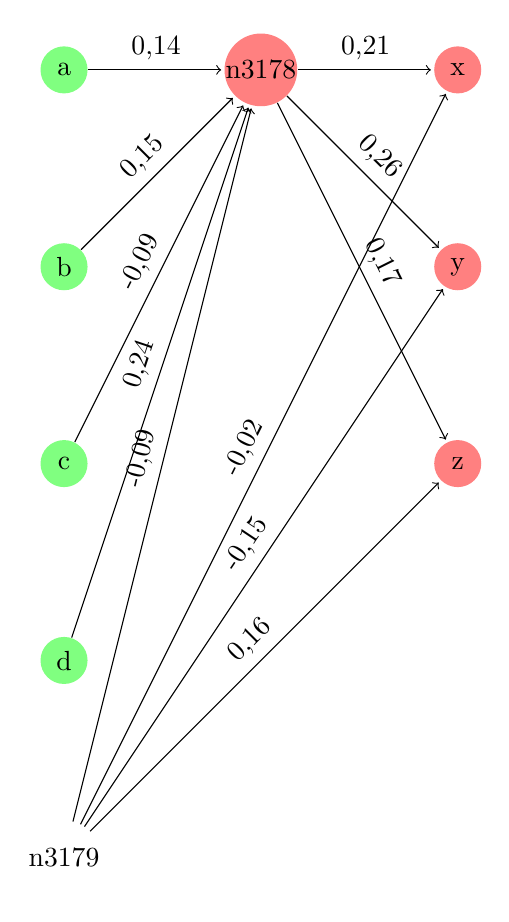
\begin{tikzpicture}[shorten >=1pt,->,draw=black!,node distance=2.5cm]
\tikzstyle{neuron}=[circle,fill=black!25,minimum size=17pt,inner sep=0pt]
\tikzstyle{constant}=[neuron, fill=white!50];
\tikzstyle{sigmoid}=[neuron, fill=red!50];
\tikzstyle{identity}=[neuron, fill=green!50];
\node [identity] (a) {a};
\node [identity,below of=a] (b) {b};
\node [identity,below of=b] (c) {c};
\node [identity,below of=c] (d) {d};
\node [constant,below of=d] (n3179) {n3179};
\node [sigmoid,right of=a] (n3178) {n3178};
\node [sigmoid,right of=n3178] (x) {x};
\node [sigmoid,below of=x] (y) {y};
\node [sigmoid,below of=y] (z) {z};
\path[every node/.style={sloped,anchor=south,auto=false}]
(n3178) edge node {0,26} (y)
(n3178) edge node {0,21} (x)
(n3178) edge node {0,17} (z)
(n3179) edge node {0,16} (z)
(n3179) edge node {-0,15} (y)
(n3179) edge node {-0,09} (n3178)
(n3179) edge node {-0,02} (x)
(d) edge node {0,24} (n3178)
(c) edge node {-0,09} (n3178)
(b) edge node {0,15} (n3178)
(a) edge node {0,14} (n3178)
;\end{tikzpicture}
\end{document}